\documentclass[12pt,twoside,a4paper]{book}

% Add preamble
% Language and encoding
\usepackage[utf8]{inputenc}
\usepackage[T1]{fontenc}
\usepackage[brazil]{babel}

% Additional commands to math mode
\usepackage{amsmath}

% Indent first line of first paragraph
\usepackage{indentfirst}

% Page numbering
\pagestyle{empty}

% Don't put page number on empty page
\usepackage{emptypage}

% Hypertext references
% \usepackage{hyperref}

% Remove space after a comma when it acts like a decimal separator
\usepackage{icomma}

% Enable use of colours
\usepackage[usenames,svgnames,dvipsnames]{xcolor}

% Show customised enumerate
\usepackage{enumerate}

% Support graphics
\usepackage[pdftex]{graphicx}

% Input raw text
\usepackage{verbatim}

% Include external raw PDF pages
\usepackage{pdfpages}

% Allow forcing a figure to be displayed "here"
\usepackage{float}

% Input code
\usepackage{listings} \lstset{basicstyle=\ttfamily}


% ---------------------------------------------------------------------
% Additional packages

\usepackage{setspace}    % Flexible spacing
\usepackage{makeidx}     % Index
\usepackage{tocbibind}   % Add bibliography/index/content to ToC
\usepackage{courier}     % Adobe Courier instead of Computer Modern Typewriter
\usepackage{type1cm}     % Scalable fonts
\usepackage{setspace}    % Spacing between lines
\usepackage{titletoc}
\usepackage[fixlanguage]{babelbib}
\usepackage[font=small,format=plain,labelfont=bf,up,textfont=it,up]{caption}

% Margins
\usepackage[a4paper,top=3cm,bottom=2cm,left=3cm,right=2cm]{geometry}

% Solve hyperref and chapter problem
\usepackage[all]{hypcap}

% Textual bibliography quote
\usepackage[round,sort,nonamebreak]{natbib}

% Add metadata to PDF
\hypersetup{
    pdfauthor = {Leonardo Pereira Macedo},
    pdftitle = {Desenvolvimento de um módulo para Godot},
    pdfsubject = {Trabalho de Conclusão de Curso - IME-USP},
    pdfkeywords = {software, game engine, Godot, desenvolvimento de módulo,
                   reconhecimento de voz},
    pdfpagemode = UseOutlines
}

\fontsize{60}{62}\usefont{OT1}{cmr}{m}{n}{\selectfont}

% Paragraph indent size
% \setlength{\parindent}{2cm}

% Spacing between paragraphs
% \setlength{\parskip}{0.25cm}

% ---------------------------------------------------------------------
% Nice headers

\usepackage{fancyhdr}
\pagestyle{fancy}
\fancyhf{}
\renewcommand{\chaptermark}[1]{\markboth{\MakeUppercase{#1}}{}}
\renewcommand{\sectionmark}[1]{\markright{\MakeUppercase{#1}}{}}
\renewcommand{\headrulewidth}{0pt}

% ---------------------------------------------------------------------

\urlstyle{same}  % URL with same style as text and not monospaced
\makeindex
\raggedbottom    % Disallow extra spaces in text
\fontsize{60}{62}\usefont{OT1}{cmr}{m}{n}{\selectfont}
\cleardoublepage
\normalsize

% ---------------------------------------------------------------------
% Code listing
% Ref: http://en.wikibooks.org/wiki/LaTeX/Packages/Listings

% Define code style
\lstset{
  inputencoding=utf8,
  extendedchars=true,
  commentstyle=\color{green},
  keywordstyle=\color{magenta},
  numberstyle=\small\color{gray},  % Line number font size
  stringstyle=\color{purple},
  basicstyle=\footnotesize,        % Code font size
  xleftmargin=\parindent,
  aboveskip=2\medskipamount,       % Upper margin
  breakatwhitespace=false,         % Automatic breaks at whitespace
  breaklines=true,                 % Sets automatic line breaking
  captionpos=b,                    % Caption position (b = bottom)
  keepspaces=true,
  numbers=none,                    % Where to put line numbers
  stepnumber=1,                    % Step between two line numbers
  numbersep=5pt,                   % How far line numbers are from the code
  showspaces=false,                % Show spaces adding particular underscores
  showstringspaces=false,          % Underline spaces within strings
  showtabs=false,                  % Show tabs within strings
  tabsize=2,                       % Size of tab
  frame=single,                    % Frame type around code
  framerule=0.6pt,                 % Frame size
  backgroundcolor=\color[rgb]{1.0,1.0,0.9},
  rulecolor=\color[rgb]{0.8,0.8,0.8},
  escapeinside={\%*}{*)},          % For adding a comment within the code
  % Add literates for all accents in Portuguese
  literate={á}{{\'a}}1 {é}{{\'e}}1 {í}{{\'i}}1 {ó}{{\'o}}1 {ú}{{\'u}}1 {Á}{{\'A}}1 {É}{{\'E}}1 {Í}{{\'I}}1 {Ó}{{\'O}}1 {Ú}{{\'U}}1 {à}{{\`a}}1 {À}{{\`A}}1 {â}{{\^a}}1 {ê}{{\^e}}1 {î}{{\^i}}1 {ô}{{\^o}}1 {û}{{\^u}}1 {Â}{{\^A}}1 {Ê}{{\^E}}1 {Î}{{\^I}}1 {Ô}{{\^O}}1 {Û}{{\^U}}1 {ã}{{\~a}}1 {õ}{{\~o}}1 {Ã}{{\~A}}1 {Õ}{{\~O}}1 {ç}{{\c c}}1 {Ç}{{\c C}}1
}

% =====================================================================
% Document initial pages

\begin{document}
\sloppy  % Prevents words from passing line length

\frontmatter
% Header for pages in sections before chapter 1
\fancyhead[RO]{{\footnotesize\rightmark}\hspace{2em}\thepage}
\setcounter{tocdepth}{2}
\fancyhead[LE]{\thepage\hspace{2em}\footnotesize{\leftmark}}
\fancyhead[RE,LO]{}
\fancyhead[RO]{{\footnotesize\rightmark}\hspace{2em}\thepage}
\linespread{1.25}

\pagenumbering{gobble}
\hypersetup{pageanchor=false}
\thispagestyle{empty}
\begin{center}
    \vspace*{2.3cm}
    Universidade de São Paulo \\
    Instituto de Matemática e Estatística \\
    Bachalerado em Ciência da Computação


    \vspace*{3cm}
    \large{Leonardo Pereira Macedo}


    \vspace{3cm}
    \textbf{\large{Desenvolvimento de um módulo de reconhecimento de voz \\
    para a \textit{game engine} \textit{Godot}}}


    \vskip 5cm
    \normalsize{São Paulo}

    \today
\end{center}

\newpage
\thispagestyle{empty}
  \begin{center}
    \vspace*{2.3 cm}
    \textbf{\Large{Desenvolvimento de um plugin\\
    para a \textit{game engine} Godot}}
    \vspace*{2 cm}
  \end{center}

  \vskip 2cm

  \begin{flushright}
    Monografia final da disciplina\\
    MAC0499 -- Trabalho de Formatura Supervisionado
  \end{flushright}

  \vskip 5cm

  \begin{center}
  Supervisor: Prof. Dr. Marco Dimas Gubitoso\\

  \vskip 5cm
  \normalsize{São Paulo}

  \today
  \end{center}
\pagebreak

\pagenumbering{roman}  % Begin enumerating


\hypersetup{pageanchor=true}
\pagenumbering{roman}
\onehalfspacing
\chapter*{Agradecimentos}
\addcontentsline{toc}{chapter}{Agradecimentos}

Gostaria de agradecer muito a minha família, principalmente meus pais, pelo constante apoio durante toda a minha vida universitária. Dificilmente teria conseguido arranjar forças para chegar até o final do curso se não fosse por eles.

Sou muito grato ao IME e aos professores com as quais tive aula. Pretendo levar a dedicação e ensinamentos deles pelo resto de minha vida profissional. Em especial, agradeço ao meu orientador, o professor Gubi, pelas várias reuniões e conversas ao longo do ano sobre este trabalho.

Por fim, agradeço o apoio dos poucos mas valiosos amigos que fiz durante a graduação, pois a experiência da universidade não teria sido a mesma sem a presença deles.

% ---------------------------------------------------------------------
% Portuguese

\chapter*{Resumo}

A área de \emph{games} evoluiu muito desde o início da década da 70, quando começaram
a ser comercializados. As principais causas estão relacionadas aos avanços em
diferentes áreas da Computação.

Com o passar do tempo, surgiram as \emph{game engines}: \emph{frameworks} voltados
especificamente para a criação de jogos, visando a facilitar o desenvolvimento e/ou
algumas de suas etapas.

Focaremos em uma \emph{game engine} em particular, \emph{Godot}. Por possuir código
aberto, este \emph{software} permite a extensão de suas funcionalidades através da
criação de novos módulos.

Este projeto busca implementar um módulo de reconhecimento de voz para \emph{Godot},
depois demonstrando a nova capacidade em um jogo simples desenvolvido na própria
plataforma.
\\

\noindent \textbf{Palavras-chave:} \emph{software}, \emph{game engine}, \emph{Godot},
desenvolvimento de módulo, extensão de funcionalidade.

% ---------------------------------------------------------------------
% English

\chapter*{Abstract}

Video games have evolved considerably since the beginning of the 70's, when they
started to be commercialized. The main reasons are related to several advances in
different fields of Computer Science.

Over time, \emph{game engines} started appearing: \emph{frameworks} designed
specifically to assist on game creation, simplifying the process and/or some of its
steps.

We will focus on a specific game engine, \emph{Godot}. Since it is an open source
project, it is possible to extend its funcionalities by creating new modules.

This project's goal is to implement a speech recognition module for \emph{Godot},
then showing the new feature in a simple game developed on the engine itself.
\\

\noindent \textbf{Keywords:} software, game engine, \emph{Godot}, module development,
functionality extension.


% Add list of listings to ToC
\renewcommand{\lstlistoflistings}{
\begingroup
\tocfile{\lstlistlistingname}{lol}
\endgroup
}

{
\hypersetup{linkcolor=black}
\tableofcontents
\listoffigures
\listoftables
\lstlistoflistings
}

% ---------------------------------------------------------------------
% Document main body

\mainmatter
\pagenumbering{arabic}

% Header for all pages in chapters
\fancyhead[RE,LO]{\thesection}

% Add chapters here
\chapter{Introdução}
\label{cap:introduction}

% ---------------------------------------------------------------------

\section{Motivação e objetivo}

Hoje em dia, não há como negar que o mercado de \textit{games} é um fenômeno mundial, gerando mais de US\$ 91 bilhões em 2016 \citep{gameMarket:16}. Comparado aos primeiros jogos, comercializados no início da década de 1970 \citep{gameMarketOrigin}, a evolução em diversas áreas da computação permitiu grandes avanços nos jogos criados. Inclui-se nisso a evolução dos computadores por conta da \textit{Lei de Moore} \citep{moore}, permitindo processamento mais rápido; \textit{games} em 3D e gráficos cada vez mais sofisticados e realistas devido à Computação Gráfica; e adversários sofisticados e de raciocínio rápido com a Inteligência Artificial.

Junto aos próprios jogos, as tecnologias usadas para desenvolvê-los também tiveram progressos. Em especial, temos as \emph{game engines}, que podem ser descritas como \textquotedblleft \textit{frameworks} voltados especificamente para a criação de jogos\,\textquotedblright\:\citep{gameEngine:13}. Elas oferecem diversas ferramentas para acelerar o desenvolvimento de um jogo, como maior facilidade na manipulação gráfica e bibliotecas prontas para tratar colisões entre objetos. Além disso, como eficiência é um fator essencial para manter um bom valor de FPS (\textit{Frames per Second}), as \textit{engines} costumam ter sua base construída em linguagens rápidas e compiladas, como C e C++.

Focaremos em uma \textit{game engine} em particular, \textbf{\emph{Godot}} \citep{godot}. O principal motivo de ter sido escolhida é por ser um \textit{software} de código aberto, o que permite a qualquer pessoa baixar seu código fonte e fazer modificações. Em especial, a \textit{engine} permite a criação de novos módulos para adicionar a ele novas funcionalidades.

Este trabalho visa a criar um novo módulo para \textit{Godot}. Tal extensão adicionará funções simples de reconhecimento de voz, algo ainda inexistente no \textit{software}. Feito isso, a nova funcionalidade será demonstrada em um jogo simples criado nessa \textit{engine}.

% ---------------------------------------------------------------------

\section{Organização do trabalho}

O capítulo \ref{cap:speech-recognition} aborda resumidamente reconhecimento de voz através de um olhar teórico, seguido pelo capítulo \ref{cap:hmm}, onde estuda-se um pouco de uma forma de realizar reconhecimento de voz por meio de \textit{Modelos Ocultos de Markov}.

No capítulo \ref{cap:speech-libs}, representa-se os primeiros passos para a concretização do trabalho, pois envolve a busca da melhor biblioteca de reconhecimento de voz que possa ser usada no módulo. A biblioteca escolhida, \textit{Pocketsphinx}, é estudada no capítulo \ref{cap:pocketsphinx}.

A arquitetura do \textit{Godot} é apresentada no capítulo \ref{cap:godot} a fim de se entender a lógica por trás da construção do módulo de reconhecimento de voz no capítulo \ref{cap:stt-module}. O capítulo \ref{cap:color-clutter} apresenta a criação de jogo simples, feito na própria \textit{game engine}, para demonstrar o módulo em funcionamento e suas capacidades.

% TODO: Check where the subjective chapters will be placed
O capítulo \ref{cap:conclusion} apresenta as conclusões do trabalho. Por fim, há uma parte subjetiva contendo a apreciação pessoal do TCC e uma descrição das matérias que mais ajudaram no desenvolvimento do projeto.

\chapter{Reconhecimento de voz}
\label{cap:speech-recognition}

Neste capítulo, abordaremos a parte teórica do reconhecimento de voz, sem nos preocuparmos com a forma de implementação ou sua aplicação no contexto deste trabalho. Em particular, analisaremos brevemente os principais parâmetros que influenciam seu uso.

% ---------------------------------------------------------------------

\section{Definição}

\textbf{Reconhecimento automático de voz} (ou da fala), muitas vezes referido como \textit{speech to text} (\textbf{STT}) ou \textit{automatic speech recognition} (\textbf{ASR}), é um campo multidisciplinar que envolve as áreas de Inteligência Artificial, Estatística e Linguística. Busca-se desenvolver metodologias e tecnologias para que computadores sejam capazes de captar, reconhecer e traduzir a linguagem falada para texto \citep{sttDefinition}.

% ---------------------------------------------------------------------

\section{História}

Apresentamos uma breve visão histórica de sistemas de reconhecimento de voz, desde seu início até os dias atuais. Baseamo-nos principalmente em um artigo \citep{STTHistory}.

% ---------------------------------------------------------------------

\subsection{Décadas de 50 e 60: Primeiros passos}

O primeiro sistema de reconhecimento de voz conhecido foi o \textit{Audrey}, construído em 1952 por três pesquisadores do \textit{Bell Labs}. A máquina conseguia reconhecer apenas dígitos falados por um único usuário.

10 anos depois, a IBM apresentou o \textit{Shoebox}, que reconhecia 16 palavras em inglês, entre elas os dígitos de 0 a 9. Quando captava palavras como \textit{plus}, \textit{minus} ou \textit{total}, \textit{Shoebox} instruía outra máquina de adições a realizar cálculos ou imprimir o resultado. A entrada era feita por um microfone (figura \ref{shoebox}), que convertia a voz do usuário em impulsos elétricos, classificados internamente por um circuito de medição \citep{shoebox}.

\begin{figure}[H]
  \centering
  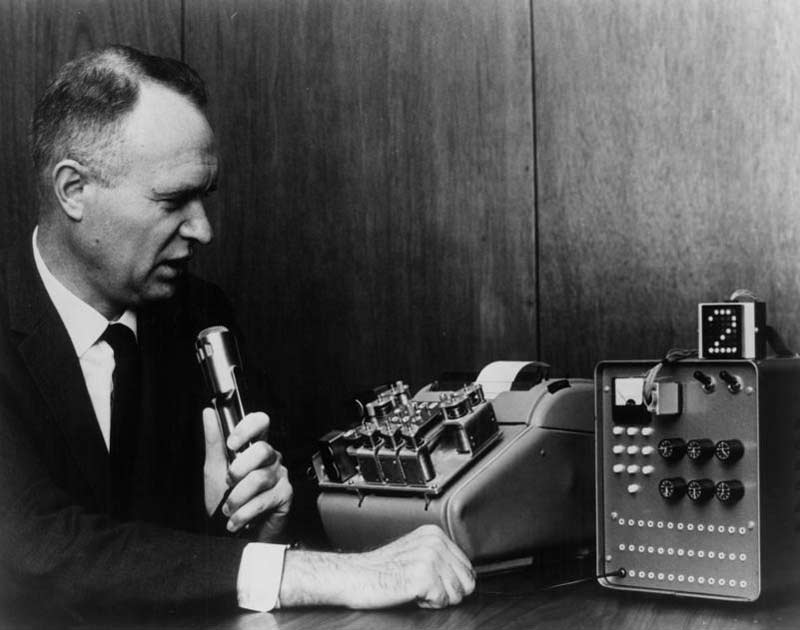
\includegraphics[width=.5\textwidth]{image/shoebox.jpg}
  \caption{Máquina \textit{Shoebox} sendo operada \citep{shoeboxImage}}
  \label{shoebox}
\end{figure}

Laboratórios nos EUA, URSS, Inglaterra e Japão começaram a desenvolver \textit{hardware} para reconhecer uma maior variedade de sons. Conseguiu-se suporte para quatro vogais e nove consoantes; um avanço notável, considerando a tecnologia da época.

% ---------------------------------------------------------------------

\subsection{Décadas de 70 e 80: Grandes avanços}

Na década de 70, o departamento de defesa dos EUA mostrou grande interesse em financiar a tecnologia de reconhecimento de voz. Tal impulso ajudou no desenvolvimento do sistema \emph{Harpy} de reconhecimento de voz pela Universidade Carnegie Mellon.

\textit{Harpy} usava um grafo para representar o domínio das palavras reconhecíveis. Um algoritmo de busca heurística, \emph{Beam Search}, era aplicado para procurar a melhor interpretação para a voz de entrada. Este algoritmo assemelha-se ao \textit{Best-First Search} (BFS), que explora um grafo através da expansão do estado mais promissor ao sair do estado presente. No entanto, sua otimização consiste em ordenar os próximos possíveis estados, através de uma heurística, antes de realizar uma expansão, o que permite prever o quão longe o estado presente está em relação ao estado meta. Com isso, o \textit{Beam Search} é caracterizado como um algoritmo guloso, que gasta menos memória quando comparado ao BFS \citep{beamSearch}.

Através de uma forma de busca mais eficiente, \textit{Harpy} conseguia entender 1011 palavras, aproximadamente o vocabulário de uma criança típica de três anos.

Sistemas de reconhecimento de voz só tiveram um avanço realmente significativo na década de 80, devido a um método estatístico denominado \textbf{Modelo Oculto de Markov} (ou \textbf{HMM}, sigla para \textit{Hidden Markov Model}). Ao invés de procurar por modelos de palavras em padrões de som, considera-se a probabilidade de um som desconhecido possuir palavras, o que acelerou o processo e tornou possível usar um vocabulário maior nos computadores.\iffalse Veremos HMM com mais detalhes no capítulo \ref{cap:hmm}.\fi

Outro modelo que ganhou bastante popularidade na mesma época foi o de redes neurais, que é efetivo para classificar palavras isoladas e fonemas individuais mas encontra problemas em tarefas envolvendo reconhecimento contínuo. Ao contrário do HMM, este método não consegue modelar bem dependências temporais. No entanto, em ambos os casos, existia a necessidade de falar pausadamente para o sistema poder melhor interpretar o usuário.

Os progressos em sistemas de reconhecimento de voz começaram a se refletir no meio comercial. Destacamos a boneca \textit{Julie} (figura \ref{julie}), comercializada em 1987 como \textit{``Finalmente, a boneca que te entende''}, pois era capaz de ser treinada para responder à voz de uma criança.

\begin{figure}[H]
  \centering
  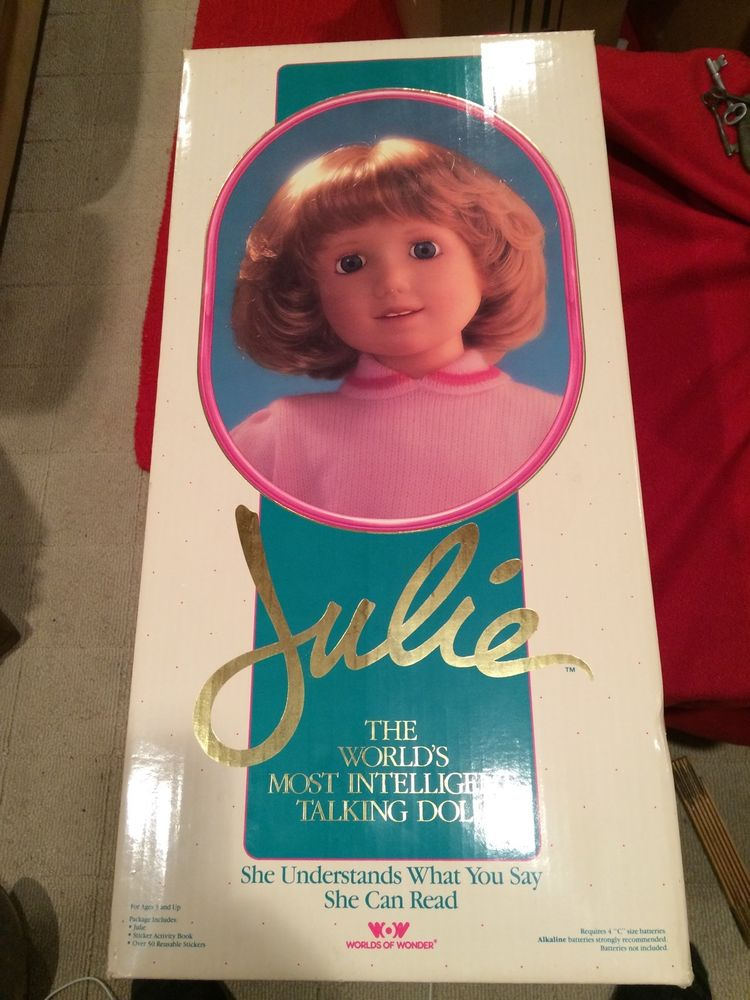
\includegraphics[width=.35\textwidth]{image/julie.jpg}
  \caption{Caixa da boneca \textit{Julie}; note, na parte inferior, a frase \textit{``Ela entende o que você diz''} \citep{julieImage}}
  \label{julie}
\end{figure}

% ---------------------------------------------------------------------

\subsection{Década de 90 até hoje: Popularização}

Na década de 90, a popularização de computadores para uso pessoal e o desenvolvimento de processadores mais rápidos permitiu que o reconhecimento de voz ficasse viável para uma quantidade maior de pessoas.

Em 1996, surgiu o primeiro portal de voz, VAL, criado pela empresa de telecomunicações norte-americana BellSouth. O sistema atendia chamadas telefônicas e respondia de acordo com a informação proferida pelo cliente.

Até o final dos anos 2000, sistemas de reconhecimento de voz pareciam ter ficado estagnados em uma acurácia de aproximadamente 80\%, e muitas aplicações eram caracterizadas pela complexidade ou dificuldade de uso se comparadas ao tradicional \textit{mouse} e teclado.

A popularidade do conceito ressurgiu com força através do aplicativo de Busca por Voz, feito pela Google para \textit{iPhone}. As duas razões para tal sucesso eram a facilidade de entrada de dados, se comparado ao teclado da plataforma, e o uso de \textit{data centers} em nuvem da Google, o que retirava a necessidade de um poderoso processamento nos \textit{iPhones} em si. Com isso, mostrava-se que era possível contornar duas das principais limitações de sistemas de voz: a disponibilidade de dados e a dificuldade de processá-los eficientemente.

A evolução na tecnologia de reconhecimento de voz foi tamanha que, atualmente, é inegável seu impacto em nosso dia a dia. Um celular moderno consegue captar palavras ou pequenas frases de seu usuário dentre um enorme vocabulário para fazer buscas na Internet, tocar uma música ou fazer uma ligação. Alguns países usam reconhecimento de voz para autenticar a identidade de alguém por telefone, com o objetivo de evitar fornecer dados pessoais pelo mesmo. Também há usos em transportes, na área médica e para fins educativos, muitas vezes acentuados pela maior facilidade em se falar um comando comparado ao uso de um teclado ou interface gráfica.

% ---------------------------------------------------------------------

\section{Componentes de um sistema genérico}
\label{sttComponents}

A figura \ref{generic-stt} apresenta os três componentes de um sistema genérico envolvendo STT \citep{sttComponentsParameters}:

\begin{itemize}
\item O \textbf{usuário} do sistema, que codifica um comando através de sua voz;

\item O \textbf{dispositivo} de STT, que converte a mensagem falada para um formato interpretável;

\item O \textbf{software de aplicação}, que recebe a saída do dispositivo e realiza uma ação apropriada.
\end{itemize}

\begin{figure}[H]
  \centering
  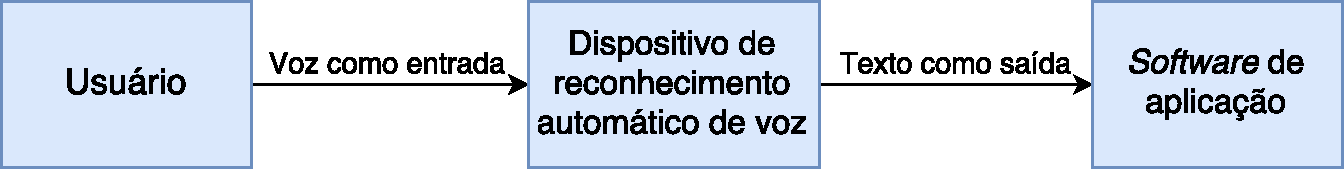
\includegraphics[width=.9\textwidth]{image/generic-stt.pdf}
  \caption{Sistema genérico de reconhecimento automático de voz \citep{sttComponentsParameters}}
  \label{generic-stt}
\end{figure}

% ---------------------------------------------------------------------

\section{Principais termos}
\label{sttMainTerms}

De acordo com \citep{sttComponentsParameters} e \citep{sttBasics}, apresentamos, a seguir, os termos mais recorrentes em sistemas de reconhecimento de voz. Também detalhamos seus parâmetros principais, que atuam sobre sua forma de funcionamento, eficiência e acurácia. A influência destes fatores varia de acordo com o tipo de aplicação que se deseja construir.

% ---------------------------------------------------------------------

\subsection{Fluência}

A fluência está relacionada à forma de se comunicar com o sistema. Tipicamente, a fala do usuário pode ser feita através de:

\begin{itemize}
\item \textbf{Palavras isoladas}, com pausas entre elas;
\item \textbf{Palavras conectadas}, que são concatenadas sem pausas;
\item \textbf{Fala contínua}, onde o fluxo de palavras é semelhante a uma fala natural.
\end{itemize}

% ---------------------------------------------------------------------

\subsection{Dependência do usuário}

A dependência ou não do usuário classifica os sistemas em dois grupos:

\begin{itemize}
\item Os sistemas \textbf{dependentes} (\textit{speaker-dependent}), caracterizados pelo \emph{treinamento} feito pelo usuário. Isto é, são computadores que analisam e se adaptam aos padrões particulares da fala captada, resultando em uma maior acurácia. Geralmente, o usuário deve ler algumas páginas de texto para a máquina antes de iniciar o uso do sistema. Esta variante é comumente escolhida em casos particulares, onde um número limitado de palavras deve ser reconhecido com bastante precisão \citep{speakerDependency}.

\item Os sistemas \textbf{independentes} (\textit{speaker-independent}), que são desenvolvidos para reconhecer a voz de qualquer pessoa e não requerem treinamento. É a melhor opção para aplicações interativas que usam voz, já que não é viável fazer com que os usuários leiam páginas de texto antes do uso, ou para sistemas usados por diferentes pessoas. Sua desvantagem é a acurácia menor se comparado ao reconhecimento dependente; para contornar isso, costuma-se limitar o vocabulário reconhecido pelo sistema \citep{speakerDependency}.
\end{itemize}

% ---------------------------------------------------------------------

\subsection{Vocabulário}

O vocabulário representa as palavras reconhecidas pelo sistema. Seu tamanho pode ser pequeno (menor que 20 palavras) até muito grande (mais de 20 mil palavras), sendo diretamente proporcional à velocidade do reconhecimento. Além disso, a similaridade entre a pronúncia de algumas palavras pode afetar a acurácia, uma vez que a distinção entre elas torna-se mais complicada.

% ---------------------------------------------------------------------

\subsection{\textit{Utterance}}

O termo \textit{utterance} não possui uma tradução exata no contexto de reconhecimento de voz, embora possa ser interpretado como \textit{``pronunciamento, elocução''}. Refere-se à vocalização (fala) de uma ou mais palavras, pronunciadas de forma contínua e terminando com uma pausa clara, que possuem um significado único ao computador. Em outras palavras, \textit{utterances} são o conteúdo entendido pelo sistema após receber a fala do usuário.

Ao voltarmos para o sistema genérico de reconhecimento de voz apresentado na seção \ref{sttComponents}, notaremos que a interpretação de \textit{utterances} representa a saída produzida pelo dispositivo de STT.

% ---------------------------------------------------------------------

\subsection{Taxa de erro por palavra}
\label{word-error-rate}

A taxa de erro por palavra (\textit{word error rate}, ou $WER$) é uma métrica de desempenho de um sistema de reconhecimento de voz \citep{wordErrorRate}.

Suponha que tenhamos o texto de referência $\tau$, correspondente ao que o usuário falou, e o texto $\tau'$ de hipótese, que foi gerado pelo sistema STT. O reconhecimento de voz pode levar a diferentes interpretações nas $N$ palavras de $\tau$, levando a um $\tau'$ diferente. Em particular, costuma haver um certo número $I$ de palavras inseridas, uma quantidade $D$ de palavras removidas e um valor $S$ de palavras substituídas.

Exemplificando, seja $\tau$ = \textit{``Gosto de chocolate''} e $\tau'$ = \textit{``Gosto chocolate''}. Houve uma remoção por conta da preposição \textit{``de''} ter sido eliminada pelo sistema de reconhecimento de voz, então $D = 1$.

A taxa de erro $WER$, geralmente expressa como uma porcentagem, é dada pela equação \ref{wer-equation}. Um valor elevado para esta métrica significa que a qualidade do reconhecimento de voz está ruim.

\begin{equation}
\label{wer-equation}
WER =  \frac{I + D + S}{N}
\end{equation}

% ---------------------------------------------------------------------

\subsection{Parâmetros ambientais}

Parâmetros ambientais referem-se a fatores externos ao sistema que podem interferir no reconhecimento de voz. Destacam-se:

\begin{itemize}
\item A \textbf{relação sinal/ruído}, que avalia a intensidade média do sinal recebido em relação ao ruído de fundo, tipicamente medido em decibéis (dB). Quanto menor a taxa, maior a dificuldade no reconhecimento de voz.

\item O \textbf{próprio usuário}, o que inclui o volume de sua voz, a velocidade com que fala e até mesmo sua condição psicológica: o nível de estresse de um piloto sob ataque em uma aeronave é diferente de alguém simplesmente querendo ouvir uma música, por exemplo.
\end{itemize}

\chapter{Modelo Oculto de Markov}
\label{cap:hmm}

\chapter{Bibliotecas para Reconhecimento de Voz}
\label{cap:speech-libs}

A seguir, veremos o primeiro item necessário para atingirmos o objetivo final: uma biblioteca que fará o reconhecimento de voz dentro do módulo.

Uma implementação do zero fugiria do tema deste trabalho, pois seria necessário aprender sobre reconhecimento de padrões voltado a sons e outros tópicos relacionados a Inteligência Artificial. A outra opção existente, e a que seguiremos, é procurar por uma biblioteca existente e aprender a manejá-la.

Analisaremos quais as características necessárias e desejáveis na biblioteca ideal, e estudaremos a que melhor se adequa ao nosso objetivo dentre as opções existentes.

% ---------------------------------------------------------------------

\section{Considerações iniciais}

Recordemos os principais componentes para reconhecimento de voz, apresentados na seção \ref{sttComponents}. No contexto do módulo de reconhecimento de voz para \textit{Godot}, as seguintes associações surgem naturalmente:

\begin{itemize}
\item O \textbf{usuário} representa tipicamente o \textbf{jogador}, que interage parcialmente ou totalmente com o jogo por meio de comandos de voz.

\item O \textbf{dispositivo de STT} corresponde ao \textbf{módulo de reconhecimento de voz}, objetivo principal deste trabalho. Esta componente é usada pelo jogo para converter a fala do jogador em texto.

\item O \textbf{software de aplicação} é o \textbf{jogo} em si, feito em \textit{Godot}, que recebe indiretamente os comandos do usuário e realiza ações apropriadas.
\end{itemize}

% ---------------------------------------------------------------------

\section{A biblioteca ideal}
\label{idealLibrary}

Realçamos novamente que o módulo de reconhecimento de voz será usado diretamente em jogos. Tal contexto automaticamente nos leva a pensar em diversas características que a biblioteca ideal deve possuir.

% ---------------------------------------------------------------------

\subsection{Características obrigatórias}

Em ordem decrescente de importância, temos:

\begin{enumerate}
\item \textbf{Ter código aberto e licença permissiva:} Justifica-se pela integração da biblioteca em uma \textit{game engine} de código aberto. A importância é ainda maior se levarmos em conta que jogos com fins comerciais podem ser produzidos em \textit{Godot}.

\item \textbf{Ser eficiente (rápida):} Já foi mencionado que o módulo de reconhecimento de voz será usado em uma \textit{game engine}. Um jogo é um \textit{software} onde tipicamente a eficiência é de extrema importância, pois costuma envolver a renderização de cenas várias vezes por segundo. Devido a isso, surge a necessidade da biblioteca ser \emph{rápida} para não afetar negativamente a experiência do jogador.

\item \textbf{Reconhecer inglês:} O inglês possui presença constante em cenários de computação. Portanto, é a única língua que a biblioteca deve obrigatoriamente oferecer suporte.

\item \textbf{Não ser pesada:} Não é desejável ter uma biblioteca que ocupe muito espaço em disco (o que poderia aumentar o tamanho do jogo que a utiliza) e memória (aspecto relacionado diretamente à eficiência).
\end{enumerate}

% ---------------------------------------------------------------------

\subsection{Características desejáveis}

Em ordem decrescente de importância, temos:

\begin{enumerate}
\item \textbf{Ser multiplataforma:} \textit{Godot} possibilita exportar jogos para diferentes plataformas, dentre elas Windows, MacOS, Unix, Android e iOS \citep{godotDeployPlatforms}. Uma biblioteca que possa ser compatível com o maior número possível destes sistemas operacionais tornaria o módulo de reconhecimento de voz mais flexível para a produção de jogos em diferentes ambientes.

\item \textbf{Reconhecer diferentes línguas:} Apesar da obrigatoriedade do inglês, a possibilidade de usar diferentes línguas aumentaria a versatilidade do módulo. Tal característica é acentuada ao notarmos que muitos jogos, hoje em dia, oferecem a possibilidade de alterar a língua.

\item \textbf{Ser implementada em C/C++:} Conforme veremos na seção \ref{cap:godot}, \textit{Godot} possui toda a sua base escrita em C++, linguagem também usada para a criação de módulos. A implementação da biblioteca na mesma linguagem ajudaria a simplificar problemas de compatibilidade. Eventualmente, C também é uma opção viável por ser aceita pela linguagem sucessora.
\end{enumerate}

% ---------------------------------------------------------------------

\section{Bibliotecas viáveis}

Realizou-se uma pesquisa por bibliotecas de reconhecimento de voz que sigam o máximo de características possíveis propostas na seção \ref{idealLibrary}. O artigo \citep{sttLibs} sintetiza razoavelmente bem os resultados da busca. A seguir, destacamos as quatro bibliotecas mais notáveis encontradas:

\begin{itemize}
\item \textbf{Kaldi} \citep{kaldi}: É a biblioteca mais recente da lista, com seu código publicado em 2011. Escrita em C++, é tida como uma biblioteca para pesquisadores de reconhecimento de voz.

\item \textbf{CMUSphinx} \citep{cmusphinx}: Desenvolvida pela \textit{Carnegie Mellon University}, possui diversos pacotes para diferentes tarefas e aplicações. O pacote principal é escrito em Java. Existe também a variante \emph{Pocketsphinx}, com características interessantes para este trabalho: é escrita em C, possuindo maior velocidade e portabilidade que a biblioteca original.

\item \textbf{HTK} \citep{htk}: Desenvolvida pela \textit{Cambridge University Engineering Department}, HTK é uma sigla para \textit{Hidden Markov Model Toolkit}. É escrita em C, com novas versões sendo lançadas consistentemente.

\item \textbf{Simon} \citep{Simon}: Popular para Linux e escrita em C++, Simon utiliza \textit{CMUSphinx}, \textit{HTK} e \textit{Julius} internamente. Não havia suporte para \textit{MacOS} até abril de 2017.
\end{itemize}

% TODO: Explain better each library and the comparison article
Um artigo de 2014 comparou \emph{Kaldi}, \emph{CMUSphinx} e \emph{HTK} em relação a precisão e tempo gasto \citep{compareSpeech}. \emph{Kaldi} obteve resultados vastamente superiores; \emph{CMUSphinx} obteve bons resultados em pouco tempo; \emph{HTK} precisou de muito mais tempo e treino para conseguir resultados na ordem dos outros dois.

% ---------------------------------------------------------------------

\section{\textit{Pocketsphinx}, a biblioteca escolhida}

% TODO: Write this section

\chapter{\textit{Pocketsphinx}}
\label{cap:pocketsphinx}

Neste capítulo, analisaremos mais a fundo a biblioteca \textit{Pocketsphinx}, incluindo seu funcionamento, instruções para usá-la de forma básica e passos para compilação a partir do código fonte.

Supõe-se que o usuário esteja usando um sistema operacional \textit{Unix}, e que possua acesso a privilégios administrativos para a realização de alguns passos. Recomenda-se que o leitor possua um microfone à disposição no computador, podendo ser embutido ou externo, para melhor aproveitamento.

Todas as instruções e comandos apresentados foram originalmente realizados no sistema \texttt{Ubuntu 16.04 LTS, 64-bit} do autor.

% ---------------------------------------------------------------------

\section{Funcionamento}

O funcionamento das bibliotecas do projeto \textit{CMUSphinx}, incluindo-se a \textit{Pocketsphinx}, pode ser resumido por três grandes passos:

\begin{itemize}
\item A configuração inicial de arquivos a serem usados pela biblioteca, como o dicionário.
\item A captura de áudio de voz, separando-a em \textit{utterances}.
\item A busca, para cada \textit{utterance}, da melhor combinação de palavras do dicionário que se assemelhe a ela.
\end{itemize}

Definimos, abaixo, alguns conceitos numa ordem que nos proporcione um melhor entendimento das etapas descritas.

% ---------------------------------------------------------------------

\subsection{Fonema}

Um \textbf{fonema} é a menor unidade de som em uma língua.

O leitor poderia pensar que uma palavra é uma sequência de fonemas, mas tal definição esconde diversas complexidades: há sons que surgem na transição entre palavras e variantes linguísticas na pronúncia do falante, por exemplo. Devido a isso, surgem termos como \textit{difonemas} e \textit{trifonemas}, que tratam de fonemas consecutivos para levar em conta o contexto em que o som é captado.

% ---------------------------------------------------------------------

\subsection{Vetor de características}

Em aprendizado de máquina, uma \textbf{característica} é uma quantidade que descreve algum exemplo.

No contexto de reconhecimento de voz, CMUSphinx divide as \textit{utterances} em quadros (\textit{frames}) de aproximadamente 10 ms de comprimento. Através de uma função complexa, extraem-se 39 números -- características -- para representar a \textit{utterance}; juntos, eles formam o \textbf{vetor de características}.

% ---------------------------------------------------------------------

\subsection{Modelo}
\label{pocketsphinx-models}

Um \textbf{modelo} é uma simplificação, onde reduz-se o que se quer modelar às suas características mais importantes. Neste caso, falamos de um modelo de reconhecimento de voz: como tratar as transições entre os quadros em que se divide o áudio capturado?

A solução encontrada pelo projeto CMUSphinx foi utilizar o Modelo Oculto de Markov (\textit{Hidden Markov Model}, ou HMM, \iffalse conforme visto na seção \ref{cap:hmm})\fi para tratar a fala gravada como uma sequência de estados que transitam entre si com certa probabilidade.

Buscam-se os estados do HMM que levam à maior probabilidade no vetor de características. Para isso, três modelos, alimentados à biblioteca na forma de arquivos externos, são usados:

\begin{itemize}
\item \textbf{Modelo acústico}: Conjunto de arquivos que contém propriedades acústicas para detectores de fonemas. Define os vetores de características mais prováveis para cada unidade de som, além de determinar a criação de uma sequência de fonemas para um dado contexto. Este modelo costuma vir na forma de vários arquivos. Possui alta dependência com a língua na qual se realiza o reconhecimento de voz.

\item \textbf{Dicionário fonético}: Arquivo texto responsável por mapear palavras em fonemas, que devem existir segundo o modelo acústico. Um mapeamento perfeito é praticamente impossível; devido a variantes linguísticas e outros fatores, não há como adicionar todas as diferentes formas de se pronunciar uma palavra.

Um exemplo de uma linha de um dicionário em inglês seria:

\begin{center}
\texttt{yellow Y EH L OW}
\end{center}

\item \textbf{Modelo de linguagem}: Arquivo que formaliza uma sintaxe para a linguagem a ser reconhecida. Sua principal finalidade é diminuir o espaço de busca nas palavras, descartando-se palavras improváveis no áudio capturado e melhorando a acurácia.
\end{itemize}

% ---------------------------------------------------------------------

\subsection{Palavras-chave}
\label{pocketsphinx-keywords}

Dentre várias formas diferentes de busca, \textit{CMUSphinx} também oferece suporte para reconhecimento de voz por palavras-chave. Ao invés de usar um modelo de linguagem, fornece-se à biblioteca um arquivo de palavras ou frases a qual se quer detectar, juntamente com um limiar de detecção. Qualquer som capturado que não se encaixar no arquivo ou cujo limiar calculado for baixo demais será descartado.

Um exemplo de linha no arquivo de palavras-chave está a seguir: cada palavra deve vir seguida de seu limiar. Destaca-se que este valor deve vir isolado entre caracteres \texttt{``/''}.

\begin{center}
\texttt{yellow /1e-6/}
\end{center}

% ---------------------------------------------------------------------

\section{Compilação}
\label{sphinxCompile}

Apresentamos instruções, em \textit{Bash}, para baixar e compilar a biblioteca \textit{Pocketsphinx}. Os passos foram baseados nas instruções em \citep{pocketsphinxInstallUse}.

Antes de começar, instale as seguintes dependências em seu sistema:

\begin{center}
\footnotesize\texttt{gcc, automake, autoconf, libtool, bison, swig, python-dev, pulseaudio}
\end{center}

Em um sistema \emph{Ubuntu}, por exemplo, digitaria-se no terminal:

\begin{lstlisting}[language=Bash]
$ sudo apt-get install gcc automake autoconf libtool bison swig \
  python-dev pulseaudio
\end{lstlisting}

% ---------------------------------------------------------------------

\subsection{Pacote \textit{Sphinxbase}}
\label{sphinxbaseCompile}

O pacote \textbf{Sphinxbase} oferece funcionalidades comuns a todos os projetos \textit{CMUSphinx}. Siga as instruções abaixo para compilá-lo.

\begin{enumerate}
\item Clone o repositório do \textit{Sphinxbase}.

\begin{lstlisting}[language=Bash]
$ git clone https://github.com/cmusphinx/sphinxbase
\end{lstlisting}

\item Dentro do diretório \texttt{sphinxbase/} criado pelo passo anterior, execute o \textit{script} \texttt{autogen.sh} para gerar o arquivo \texttt{configure}:

\begin{lstlisting}[language=Bash]
$ ./autogen.sh
\end{lstlisting}

\item Execute o \textit{script} \texttt{configure} criado no último passo:

\begin{lstlisting}[language=Bash]
# Padrão
$ ./configure

# Plataformas sem aritmética de ponto flutuante
$ ./configure ---enable-fixed ---without-lapack
\end{lstlisting}

Note que qualquer dependência ausente no sistema (por exemplo, o pacote \texttt{swig}) será notificada ao usuário neste passo. Se a execução ocorrer sem problemas, um \texttt{Makefile} será gerado.

\item Compile o \textit{Sphinxbase} através do \texttt{Makefile}:

\begin{lstlisting}[language=Bash]
$ make
\end{lstlisting}

\end{enumerate}

% ---------------------------------------------------------------------

\subsection{Pacote \textit{Pocketsphinx}}
\label{pocketsphinxCompile}

O pacote \textbf{Pocketsphinx} contém as funcionalidades de reconhecimento de voz em si que nos interessam para este trabalho. Siga as instruções abaixo para compilá-lo.

\begin{enumerate}
\item Clone o repositório do \textit{Pocketsphinx}, o que criará o diretório \texttt{pocketsphinx/}.

\begin{lstlisting}[language=Bash]
$ git clone https://github.com/cmusphinx/pocketsphinx
\end{lstlisting}

\item Certifique-se que as pastas \texttt{sphinxbase/} e \texttt{pocketsphinx/} estejam no mesmo diretório, pois \textit{Pocketsphinx} usa o caminho \texttt{../} para procurar pelo pacote \textit{Sphinxbase}.

\item Dentro do diretório \texttt{pocketsphinx/}, execute o \textit{script} \texttt{autogen.sh} para gerar o arquivo \texttt{configure}:

\begin{lstlisting}[language=Bash]
$ ./autogen.sh
\end{lstlisting}

\item Execute o \textit{script} \texttt{configure} criado no último passo:

\begin{lstlisting}[language=Bash]
$ ./configure
\end{lstlisting}

Note que qualquer dependência ausente no sistema será notificada ao usuário neste passo. Se a execução ocorrer sem problemas, um \texttt{Makefile} será gerado.

\item Compile o \textit{Pocketsphinx} através do \texttt{Makefile}:

\begin{lstlisting}[language=Bash]
$ make
\end{lstlisting}

\end{enumerate}

% ---------------------------------------------------------------------

\subsection{Teste de verificação}

Para verificar se a compilação feita nas subseções \ref{sphinxbaseCompile} e \ref{pocketsphinxCompile} ocorreu corretamente, recomenda-se fazer um teste de reconhecimento de voz contínuo com o binário \texttt{pocketsphinx\_continuous}, criado na compilação do \textit{Pocketsphinx}. Nesta verificação, o usuário fala uma palavra ou uma frase curta, em inglês, em seu microfone. Quando um silêncio é detectado, o programa analisa o \textit{utterance} obtido e imprime na tela o texto que calculou ser a melhor interpretação.

No diretório onde encontram-se as pastas \texttt{sphinxbase/} e \texttt{pocketsphinx/}, execute o conteúdo da listagem \ref{sphinxTest}.

\lstinputlisting[
  language=Bash,
  basicstyle=\scriptsize,
  caption={Comandos para teste de reconhecimento de voz contínuo usando \textit{Pocketsphinx}},
  label={sphinxTest}]
  {listing/run-sphinx-continuous.sh}

O programa imediatamente irá imprimir uma lista de seus parâmetros e seus respectivos valores. Depois, avisará ao usuário que está pronto para receber a entrada de voz por meio de uma linha terminada em \texttt{Ready....}

A listagem \ref{sphinx123} representa uma saída resumida ao se falar \texttt{``one two three''} no microfone. Os caracteres \texttt{[..]} representam uma ou mais linhas omitidas.

\lstinputlisting[
  basicstyle=\scriptsize,
  numbers=left,
  caption={Saída do \texttt{pocketsphinx\_continuous} ao se falar \texttt{``one two three''}},
  label={sphinx123}]
  {listing/sphinx-continuous-123.txt}

Uma interpretação detalhada de toda a saída exige um estudo maior em reconhecimento de voz e na biblioteca \textit{Pocketsphinx} em si. No entanto, destacamos alguma informações, como o número de palavras reconhecidas (linhas 4 e 8) e a quantidade de \textit{senones} (detectores curtos de sons para trifonemas) captadas.

% ---------------------------------------------------------------------

\section{Estruturas e tipos importantes}
\label{pocketsphinx-structs}

Feita a compilação da biblioteca, começaremos a analisar as ferramentas que oferece para implementação de reconhecimento de voz. Ressaltamos que a implementação dos pacotes \textit{Sphinxbase} e \textit{Pocketsphinx} é feita na linguagem \textit{C}.

Dentre os tipos de dados oferecidos pelos pacotes \textit{Sphinxbase} e \textit{Pocketsphinx}, destacamos três, a seguir, que serão importantes para um experimento que faremos em breve.

% ---------------------------------------------------------------------

\subsection{Configuração: \texttt{cmd\_ln\_t}}

A \textit{struct} \texttt{cmd\_ln\_t}, definida no pacote \textit{Sphinxbase}, representa uma variável de configuração \citep{pocketsphinxInstallUse}. Ela é fornecida a outros tipos de dados em \textit{Pocketsphinx}; informa-se, por exemplo, os arquivos a serem usados (dicionário, modelo acústico, etc.) e se reconhecimento usará um arquivo de áudio ou será feito na hora.

Um ponteiro pode ser alocado e gerenciado com a função \texttt{cmd\_ln\_init()}, devendo-se liberá-lo posteriormente com uma chamada a \texttt{cmd\_ln\_free\_r()}.

Um dos parâmetros existentes neste tipo de configuração é o nome do microfone, no contexto do sistema do usuário. Não conseguimos encontrar uma forma de se obter, em tempo de execução, os nomes dos microfones disponíveis em um sistema \textit{Unix}. Percebemos, também, que seria bastante complicado desenvolver uma solução que funcionasse independentemente do sistema operacional. Portanto, escolhemos passar o nome do microfone como \texttt{NULL}, o que leva \textit{Pocketsphinx} a sempre utilizar o microfone padrão do computador, seja qual for a plataforma em que ele está.

% ---------------------------------------------------------------------

\subsection{Gravação: \texttt{ad\_rec\_t}}

A \textit{struct} \texttt{ad\_rec\_t} está definida no pacote \textit{Sphinxbase} e tem como objetivo gravar som de alguma entrada de voz \citep{pocketsphinxInstallUse}. Seu uso é vital na implementação de reconhecimento de voz contínuo, através do microfone do usuário.

Aloca-se um ponteiro para este tipo com a função \texttt{ad\_open\_dev()}, cujos parâmetros são um ponteiro para um tipo de configuração \texttt{cmd\_ln\_t} e a taxa de amostragem por segundo. O ponteiro do gravador deve ser liberado posteriormente  com \texttt{ad\_close()}.

As três funções mais importantes para manipulação de um \texttt{ad\_rec\_t} são explicadas abaixo. Todas elas retornam um inteiro diferente de 0 no caso de um erro ocorrer.

\subsubsection{\texttt{int ad\_start\_rec(recorder)}}

Inicia a gravação no seu argumento \texttt{ad\_rec\_t *recorder}.

\subsubsection{\texttt{int ad\_read(recorder, buffer, size)}}

Lê o áudio gravado em \texttt{ad\_rec\_t *recorder} desde a última chamada desta função para este argumento. Guarda-se o áudio lido em um \textit{buffer} do tipo inteiro, que possui o tamanho \texttt{size} especificado.

\subsubsection{\texttt{int ad\_stop\_rec(recorder)}}

Termina a gravação no seu argumento \texttt{ad\_rec\_t *recorder}.

% ---------------------------------------------------------------------

\subsection{Decodificação: \texttt{ps\_decoder\_t}}

A \textit{struct} \texttt{ps\_decoder\_t}, definida no pacote \textit{Pocketsphinx}, representa um decodificador de áudio para texto \citep{pocketsphinxInstallUse}. Toda a lógica por trás de reconhecimento de voz, portanto, é tratada por funções ligadas a este tipo.

Cria-se um ponteiro para um decodificador com a função \texttt{ps\_init()}, que recebe um tipo de configuração \texttt{cmd\_ln\_t} como seu único argumento. A memória alocada deve ser liberada após seu uso com a função \texttt{ps\_free()}.

Suas funções mais importantes para manipulação são explicadas a seguir. Todas as funções do tipo \texttt{int} retornam um inteiro diferente de 0 no caso de um erro ocorrer.

\subsubsection{\texttt{int ps\_start\_utt(decoder)}}

Inicializa o processamento para \textit{utterance} no \texttt{ps\_decoder\_t *decoder} indicado.

\subsubsection{\texttt{int ps\_process\_raw(decoder, buffer, size, no\_search, full\_utt)}}

Usa-se \texttt{ps\_decoder\_t *decoder} para decodificar o áudio guardado no \textit{buffer} de tamanho especificado. Os dois parâmetros restantes representam pequenas otimizações possíveis: \texttt{no\_search} realiza parcialmente o reconhecimento para usar menos processamento, e \texttt{full\_utt} considera o \textit{buffer} inteiro como um \textit{utterance}.

\subsubsection{\texttt{bool ps\_get\_in\_speech(decoder)}}

Retorna \texttt{true} se o \texttt{ps\_decoder\_t *decoder} fornecido tiver decodificado algo, ou \texttt{false} caso contrário. Esta função só deve ser chamada após um \texttt{ps\_process\_raw()}.

\subsubsection{\texttt{char * ps\_get\_hyp(decoder, \&score)}}

Retorna a hipótese (isto é, o termo mais provável) para um \texttt{ps\_decoder\_t *decoder} que foi processado anteriormente com \texttt{ps\_process\_raw()}. Opcionalmente, se um modelo de língua está sendo usado, pode-se passar a referência de um inteiro como segundo argumento para obter a avaliação (\textit{score}) recebida para a hipótese.

\subsubsection{\texttt{int ps\_stop\_utt(decoder)}}
Termina o processamento para \textit{utterance} no \texttt{ps\_decoder\_t *decoder} indicado.

% ---------------------------------------------------------------------

\section{Implementação de reconhecimento contínuo}
\label{stt-continuous-algorithm}

O reconhecimento contínuo de palavras-chave foi implementado com base no código presente em \citep{pocketsphinxMicLoop}. Apresentamos, na listagem \ref{ps-stt-loop}, a função que implementa o laço central do algoritmo, onde repetidamente capta-se a voz do usuário para processamento e imprime-se, na tela, as palavras mais próximas ao que foi pronunciado. Removeram-se as linhas relativas a tratamento de erro para não estender demais a função.

\begin{minipage}{\linewidth}
\lstinputlisting[
  language=C,
  numbers=left,
  caption={Laço de reconhecimento de voz usando-se as ferramentas de \textit{Pocketsphinx}},
  label={ps-stt-loop}]
  {listing/ps-stt-loop.c}
\end{minipage}

As linhas 2 a 9 correspondem à inicialização de variáveis, do gravador e do decodificador. Assume-se, inicialmente, que não estamos no meio de um \textit{utterance} através de \texttt{utt\_started = false} (linha 3).

O laço de reconhecimento de voz começa na linha 11, e usa a seguinte lógica:

\begin{itemize}
\item \textbf{Linhas 12-14}: O áudio de entrada é capturado, e seus dados são processados pelo decodificador.

\item \textbf{Linhas 16-18}: Se foi possível decodificar alguma palavra do usuário, significa que estamos diante de um \textit{utterance}. Em outras palavras, o usuário está falando algo. Coloca-se \texttt{utt\_started = true}.

\item \textbf{Linhas 22-34}: A condição da linha 23 é oposta à que acabamos de ver anteriormente, verificando se o gravador/decodificador não detectaram mais nenhuma palavra vinda do usuário. Caso seja verdade, encerramos o \textit{utterance} atual e adquirimos sua interpretação (hipótese) através de \texttt{ps\_get\_hyp()} (linhas 26 a 28). Por fim, reiniciamos o decodificador para captar um novo \textit{utterance}, alterando \texttt{utt\_started} para \texttt{false} para refletir esta mudança (linhas 31 a 33).
\end{itemize}

O leitor talvez note que a chamada a \texttt{ad\_stop\_rec()} na linha 37 é inalcançável devido ao laço implementado não possuir condição de parada. A implementação foi feita desta forma porque a situação apresentada é um teste; em um caso mais específico, como na implementação do módulo de reconhecimento de voz, a presença de uma condição de parada é vital.


% ---------------------------------------------------------------------
% Appendix

% Header
\renewcommand{\chaptermark}[1]{\markboth{\MakeUppercase{\appendixname\ \thechapter}} {\MakeUppercase{#1}} }
\fancyhead[RE,LO]{}
\appendix

% Add appendix files here

% ---------------------------------------------------------------------
% Bibliography

\backmatter
\bibliographystyle{bib/plainnat-ime}  % Textual bibliographic quote

% Add bibliography files here
\bibliography{bib/reference}

% ---------------------------------------------------------------------
% Index

% \index{TBP|see{periodicidade região codificante}}
% \index{DSP|see{processamento digital de sinais}}
% \index{STFT|see{transformada de Fourier de tempo reduzido}}
% \index{DFT|see{transformada discreta de Fourier}}
% \index{Fourier!transformada|see{transformada de Fourier}}

% \printindex  % imprime o índice remissivo no documento

% ---------------------------------------------------------------------

\end{document}
